\documentclass[11pt]{article}

\usepackage[margin=2.5cm]{geometry}
\usepackage{booktabs}
\usepackage{array}
\usepackage{xcolor}
\usepackage{hyperref}
\usepackage{caption}
\usepackage{amsmath}
\usepackage{pgfplots}
\pgfplotsset{compat=1.18}
\usepackage{enumitem}
\usepackage{fancyhdr}

\hypersetup{
    colorlinks=true,
    linkcolor=blue!50!black,
    urlcolor=blue!50!black,
    citecolor=blue!50!black,
}

\newcommand{\code}[1]{\texttt{#1}}
\newcommand{\pp}{\,\text{pp}}

\pagestyle{fancy}
\fancyhf{}
\fancyhead[L]{Scaling Diagnosis --- Progress Report}
\fancyhead[R]{\thepage}
\renewcommand{\headrulewidth}{0.4pt}

\title{\textbf{Diagnosing the Client-Count Scaling Failure of\\ Metric-Privacy Noise Calibration}\\[0.3em]
\large Progress Report}
\author{Federated Learning + Differential Privacy Research Project}
\date{August 4, 2026}

\begin{document}
\maketitle

\begin{abstract}
\noindent
This report documents an ongoing investigation into why the
metric-privacy noise-calibration mechanism of Sáinz-Pardo~Díaz et al.\ (2026), which showed a
genuine accuracy advantage over fixed-multiplier global DP at 8 federated clients
($+6.9\pp$ homogeneous, $+12.2\pp$ non-IID), collapses or reverses at 48 clients. Two
constant-compute experimental controls were designed, implemented, and run to disentangle a
genuine scaling failure of the mechanism from a confound with per-round training budget. In the
course of this work, a chain of five real infrastructure bugs was found and fixed (a unified-memory
leak, a DataLoader worker-churn regression, a dataset-reload race, an uncaught aggregation crash,
and a methodology confound in the first control design itself). Most significantly, a
non-determinism in Apple Silicon's MPS backend was discovered and directly proven: re-running the
\emph{exact same configuration} (same seed, same hyperparameters, same code) at two different times
produced accuracy deltas of up to $53.3\pp$. This noise floor is comparable to or larger than the
effect sizes this project has been treating as findings, which means \textbf{no single-run result
produced on this machine to date --- across either constant-compute design --- can currently be
trusted at face value}. Two of the highest-priority findings have already been directly
noise-checked and both failed to hold up as stated. The report closes with the concrete next steps
required before diagnosis can resume on solid ground.
\end{abstract}

\tableofcontents

% =====================================================================
\section{Background and Research Question}
% =====================================================================

The source paper calibrates server-side differential-privacy noise by the maximum pairwise distance
between client model updates (\code{maximum\_pairwise\_model\_distance} in
\code{metricdp\_pytorch/metricdp\_strategy.py}), scaling the effective noise multiplier as
$\text{noise\_multiplier} / \text{distance}$. It reports this beating a fixed-multiplier ``global-DP''
baseline on accuracy at matched privacy, but validates the claim only at 4 clients, on one
dataset/model, with an explicitly heuristic (unproven) calibration.

Prior work in this repository established two facts that motivate this diagnosis:
\begin{itemize}[leftmargin=1.4em]
    \item At \textbf{8 clients}, sweeping the noise multiplier surfaces a genuine, previously
    unpublished effect: metric-privacy beats global-DP by $+6.9\pp$ (homogeneous) and $+12.2\pp$
    (non-IID) at $\text{noise\_multiplier}=0.05$.
    \item At \textbf{48 clients}, reusing that same $\text{noise\_multiplier}=0.05$ under a
    \emph{fixed} 20-round budget, the advantage shrinks to near zero or reverses
    (FedAvg $+0.6/+2.2\pp$, FedYogi $-1.7/-0.2\pp$), while overall accuracy drops sharply.
\end{itemize}

However, both the 8-client and 48-client sweeps hardcoded a 20-round training budget regardless of
client count, while per-client data shrinks roughly $\propto 1/n$. This confounds two hypotheses:
(a) the metric-privacy mechanism genuinely degrades as client count grows, or (b) each client is
simply under-trained at 48 clients because a fixed round budget gives it far less data per round
than at 8. \textbf{The goal of this diagnosis is to disentangle these two hypotheses} before any
mechanism redesign is attempted.

% =====================================================================
\section{Summary of Work Completed}
% =====================================================================

Work proceeded in three stages, each surfacing a problem that had to be resolved before the next
could produce trustworthy data:

\begin{enumerate}[leftmargin=1.4em]
    \item \textbf{Infrastructure hardening} (\S\ref{sec:infra}) --- five real bugs found and fixed
    while running the first sweeps, none of which touch the research question directly but all of
    which were blocking reliable data collection.
    \item \textbf{Constant-compute control design and execution} (\S\ref{sec:methodology},
    \S\ref{sec:results}) --- a first control design (v1) was implemented, run to completion (12
    combinations), and written up; a methodology flaw in that design was then identified, leading to
    a corrected second design (v2), also run to completion (12 combinations).
    \item \textbf{Measurement-noise investigation} (\S\ref{sec:mps}, \S\ref{sec:noisefloor}) ---
    comparing v1 and v2 exposed a much deeper problem than either was designed to detect: the
    training backend itself (Apple MPS) is non-deterministic across process launches even with
    every seed fixed, at a magnitude that can exceed the effect sizes being measured. This was
    root-caused, proven directly, and partially mitigated (an opt-in exact-reproducibility mode).
    Two specific findings were then re-run several times each to check whether they survive this
    noise; neither does, for different reasons.
\end{enumerate}

The net result of this work to date is not yet ``does the mechanism fail at scale'' --- it is
``the constant-compute controls needed to answer that question are built and run, but the platform
they ran on is not yet proven precise enough to trust the answer they gave.'' \S\ref{sec:status}
states this precisely.

% =====================================================================
\section{Infrastructure Fixes}
\label{sec:infra}
% =====================================================================

Running the first sweep at high client counts (48) and high round counts (240, see
\S\ref{sec:v1design}) immediately exposed problems invisible at the smaller scales used previously.
All were root-caused and fixed on \code{feature/scaling-diagnosis} before any result in this report
was collected.

\begin{description}[leftmargin=1.4em,style=nextline]
    \item[Unified-memory leak (MPS).] Apple's unified-memory caching allocator does not return
    freed tensor memory to the OS. Flower's Ray simulation backend keeps each simulated client as a
    long-lived actor process for an entire run, so on MPS this pooled-but-idle memory accumulated
    round over round within each actor and eventually exceeded total system RAM on long,
    high-round-count runs. Fixed by calling \code{torch.mps.empty\_cache()} /
    \code{torch.cuda.empty\_cache()} once per client task.
    \item[Process orphaning.] Hard-killing hung runs during debugging left \code{torch\_shm\_manager}
    and other subprocess trees re-parented to \code{init} (\code{ppid=1}), which accumulated across
    debugging iterations and independently exhausted system memory/swap. Fixed with an explicit
    cleanup pass (matched via \code{ps -eo pid,ppid,args}, filtered on \code{ppid==1}) run before
    and after every sweep combination.
    \item[DataLoader worker churn.] \code{num\_workers=2} was spawning and tearing down worker
    processes far more aggressively than expected under concurrent multi-actor load, driving CPU
    usage far above what the workload justified. Root cause was \code{num\_workers} itself (not
    \code{persistent\_workers}, which was briefly and incorrectly suspected and reverted after
    confirming it amortizes worker cost \emph{across local epochs within one round}, not across
    rounds). Fixed by defaulting to \code{num\_workers=0}.
    \item[Per-round dataset-reload race.] Evaluation artifacts were intermittently inconsistent
    with training-time metrics. Root-caused to the dataset being reloaded from disk for every
    client on every round under concurrent access; fixed with a process-level cache in
    \code{load\_data\_module()} keyed by \code{(factory\_path, cache\_dir)}.
    \item[Uncaught aggregation crash.] \code{ZeroDivisionError} in Flower's own clipping code could
    crash an entire run on a single collapsed (zero-norm) client update round. This is now caught,
    logged as a \code{metric-dp-aggregation-collapsed} flag, and the run continues --- this flag is
    used directly in the diagnostics of \S\ref{sec:v1findings}.
\end{description}

% =====================================================================
\section{Constant-Compute Methodology}
\label{sec:methodology}
% =====================================================================

\subsection{Design v1: round-scaled (superseded)}
\label{sec:v1design}

The first control scaled the number of training rounds proportionally with client count, holding
local epochs and batch size fixed at the paper's values:
\[
    \text{rounds}(n) = \text{round}\!\left(20 \cdot \frac{n}{4}\right), \qquad
    n \in \{4, 8, 48\}
\]
so that each client's total local gradient-step count over its own data stays roughly constant
across client counts (4 clients $\to$ 20 rounds; 48 clients $\to$ 240 rounds). The matrix was
narrowed to \{global-dp, metric-privacy\} $\times$ \{fedavg\} $\times$ \{homogeneous, non-IID\}
$\times$ \{4, 8, 48\} at $\text{noise\_multiplier}=0.05$ (the 8-client sweet spot) --- 12
combinations, a deliberate time-budget reduction from the full paper-reproduction grid.

\subsection{Design v2: rounds-fixed, epoch-scaled (corrected)}
\label{sec:v2design}

After analyzing v1's results (\S\ref{sec:v1findings}), a methodology flaw was identified: scaling
\emph{rounds} at fixed local epochs and batch size also scales \emph{aggregation frequency} 12$\times$
from $n{=}4$ to $n{=}48$, while shrinking each client's per-round shard 12$\times$ --- at 48 clients,
clients see only 2--4 mini-batches per local epoch and are interrupted by aggregation and
noise-injection 240 times instead of 20. Total gradient-step count is preserved, but the training
dynamics are not comparable: the same number of steps delivered as many short, frequently-interrupted
local phases is not equivalent to the same number of steps delivered as few, substantial local
phases.

The corrected design instead holds rounds fixed at the paper's value and scales \emph{local epochs}:
\[
    \text{rounds}(n) = 20 \ \text{(constant)}, \qquad
    \text{local\_epochs}(n) = \text{round}\!\left(5 \cdot \frac{n}{4}\right), \qquad
    n \in \{4, 8, 48\}
\]
This targets aggregation-frequency parity directly (every combination aggregates exactly 20 times)
rather than only total-step-count parity. The same reduced 12-combination matrix was re-run under
this design (\code{experiments/client\_scaling/sweep\_scale\_controlled\_epochs.py}, results in
\code{results/scale\_controlled\_epochs/}).

% =====================================================================
\section{Results}
\label{sec:results}
% =====================================================================

\subsection{v1: round-scaled sweep}
\label{sec:v1findings}

\begin{table}[h]
\centering
\small
\begin{tabular}{llrrrrrr}
\toprule
Partition & Privacy & $n$ & Rounds & Accuracy & Loss & F1 & Collapsed rounds \\
\midrule
homogeneous & global-dp        & 4  & 20  & 49.53\% & 1.0493  & 0.328 & n/a \\
homogeneous & global-dp        & 8  & 40  & 14.06\% & 1.2760  & 0.035 & n/a \\
homogeneous & global-dp        & 48 & 240 & 33.44\% & 0.4933  & 0.168 & n/a \\
homogeneous & metric-privacy   & 4  & 20  & 70.94\% & 1.1314  & 0.691 & 0 \\
homogeneous & metric-privacy   & 8  & 40  & 19.69\% & 54.858  & 0.065 & 14 \\
homogeneous & metric-privacy   & 48 & 240 & 14.53\% & 0.5857  & 0.142 & 0 \\
non-IID     & global-dp        & 4  & 20  & 49.53\% & 1.0484  & 0.328 & n/a \\
non-IID     & global-dp        & 8  & 40  & 25.31\% & 1.3124  & 0.102 & n/a \\
non-IID     & global-dp        & 48 & 240 & 17.19\% & 1.1151  & 0.050 & n/a \\
non-IID     & metric-privacy   & 4  & 20  & 85.47\% & 0.5427  & 0.852 & 0 \\
non-IID     & metric-privacy   & 8  & 40  & 32.66\% & 23.472  & 0.161 & 23 \\
non-IID     & metric-privacy   & 48 & 240 & 20.31\% & 0.4509  & 0.069 & 0 \\
\bottomrule
\end{tabular}
\caption{v1 (round-scaled) constant-compute sweep, all 12 combinations,
$\text{noise\_multiplier}=0.05$, fedavg, seed 42. Source: \code{results/scale\_controlled/}.}
\label{tab:v1}
\end{table}

\noindent The headline v1 comparison against the earlier fixed-20-round $n{=}48$ baseline
(\code{results/48client\_scaling}):

\begin{table}[h]
\centering
\small
\begin{tabular}{lrr}
\toprule
Partition & $\Delta$ (metric-privacy $-$ global-dp), fixed 20 rounds & $\Delta$, constant-compute (240 rounds) \\
\midrule
homogeneous & $+0.63\pp$ & $\mathbf{-18.91\pp}$ \\
non-IID     & $+2.19\pp$ & $+3.12\pp$ \\
\bottomrule
\end{tabular}
\caption{The metric-privacy advantage reverses hard for homogeneous data once the round budget is
scaled to compensate for per-client data loss; it survives, barely, for non-IID.}
\label{tab:v1-delta}
\end{table}

At face value, v1 suggested the metric-privacy advantage \emph{degrades further}, not less, once
the round-budget confound is controlled for. As detailed in \S\ref{sec:mps}--\S\ref{sec:noisefloor},
this headline result does not currently survive a direct noise check and should not be cited as
established.

\subsection{v2: rounds-fixed, epoch-scaled sweep}
\label{sec:v2findings}

\begin{table}[h]
\centering
\small
\begin{tabular}{llrrrrr}
\toprule
Partition & Privacy & $n$ & Local epochs & Accuracy & Loss & Collapsed rounds \\
\midrule
homogeneous & global-dp        & 4  & 5  & 35.78\% & 0.3699 & n/a \\
homogeneous & global-dp        & 8  & 10 & 39.38\% & 0.5683 & n/a \\
homogeneous & global-dp        & 48 & 60 & 35.47\% & 0.6191 & n/a \\
homogeneous & metric-privacy   & 4  & 5  & 30.31\% & 0.5530 & 0 \\
homogeneous & metric-privacy   & 8  & 10 & 24.22\% & 35.890 & 5 \\
homogeneous & metric-privacy   & 48 & 60 & 34.53\% & 0.6054 & 0 \\
non-IID     & global-dp        & 4  & 5  & 31.87\% & 0.5600 & n/a \\
non-IID     & global-dp        & 8  & 10 & 38.44\% & 0.5443 & n/a \\
non-IID     & global-dp        & 48 & 60 & 33.44\% & 0.6816 & n/a \\
non-IID     & metric-privacy   & 4  & 5  & 32.19\% & 0.5797 & 0 \\
non-IID     & metric-privacy   & 8  & 10 & 24.84\% & 41.621 & 7 \\
non-IID     & metric-privacy   & 48 & 60 & 37.81\% & 0.5829 & 0 \\
\bottomrule
\end{tabular}
\caption{v2 (epoch-scaled, corrected control) sweep, all 12 combinations, seed 42. Source:
\code{results/scale\_controlled\_epochs/}. \textbf{Not yet written up as a standalone report} ---
this table is the first place these numbers appear.}
\label{tab:v2}
\end{table}

\begin{table}[h]
\centering
\small
\begin{tabular}{lrrr}
\toprule
Partition & $\Delta$ at $n{=}4$ & $\Delta$ at $n{=}8$ & $\Delta$ at $n{=}48$ \\
\midrule
homogeneous & $-5.47\pp$ & $-15.16\pp$ & $-0.94\pp$ \\
non-IID     & $+0.32\pp$ & $-13.60\pp$ & $+4.37\pp$ \\
\bottomrule
\end{tabular}
\caption{v2's metric-privacy $-$ global-dp deltas. Note this does \emph{not} reproduce even the
qualitative $n{=}4$ starting point of v1 (there: large positive advantage at $n{=}4$; here: near
zero or negative) under an allegedly identical base configuration --- see \S\ref{sec:mps} for why.}
\label{tab:v2-delta}
\end{table}

% =====================================================================
\section{Critical Discovery: MPS Backend Non-Determinism}
\label{sec:mps}
% =====================================================================

\subsection{How it surfaced}

v2's $n{=}4$ baseline uses \emph{exactly} the same configuration as v1's $n{=}4$ baseline
(both hold rounds fixed at 20 and local epochs fixed at 5 by construction, since
$\text{round}(5 \cdot 4/4) = 5$) --- same seed (42), same hyperparameters, same code path. These
should be bit-for-bit reproducible runs. They are not.

\begin{table}[h]
\centering
\small
\begin{tabular}{lrrr}
\toprule
Combination & v1 accuracy & v2 accuracy & $\Delta$ \\
\midrule
homogeneous / global-dp        & 49.53\% & 35.78\% & $-13.75\pp$ \\
homogeneous / metric-privacy   & 70.94\% & 30.31\% & $-40.62\pp$ \\
non-IID / global-dp            & 49.53\% & 31.87\% & $-17.66\pp$ \\
non-IID / metric-privacy       & 85.47\% & 32.19\% & $-53.28\pp$ \\
\bottomrule
\end{tabular}
\caption{\textbf{Identical configuration, run at two different times, same seed}: all four $n{=}4$
baseline points diverge by 13.75--53.28pp. Metadata for both runs was diffed directly (num\_clients,
rounds, local\_epochs, noise\_multiplier, seed, partition, privacy, aggregation, batch\_size all
confirmed identical) --- this is not a configuration bug, it is the training backend itself failing
to reproduce.}
\label{tab:mps-proof}
\end{table}

\begin{center}
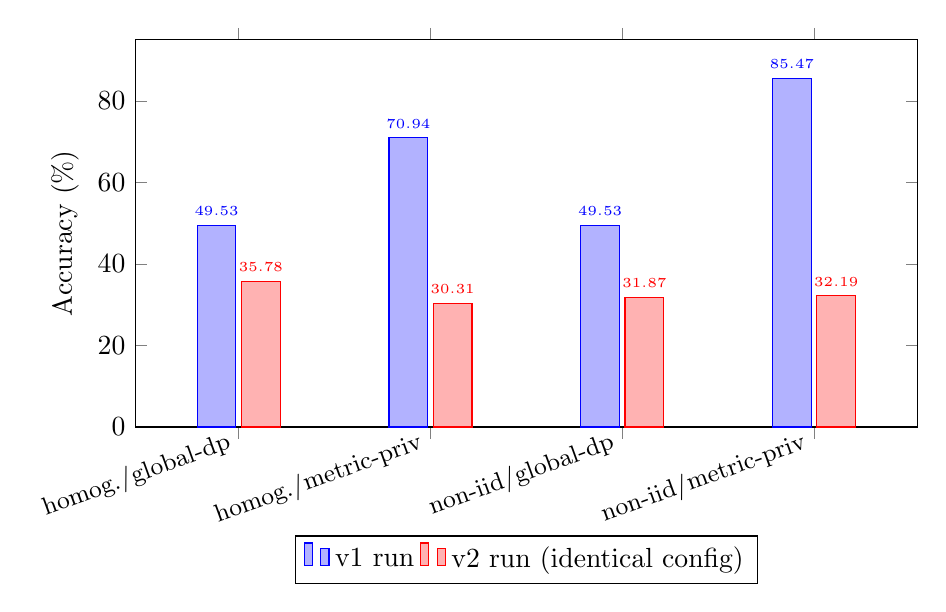
\begin{tikzpicture}
\begin{axis}[
    ybar,
    bar width=14pt,
    width=0.95\textwidth,
    height=6.5cm,
    ylabel={Accuracy (\%)},
    symbolic x coords={hom/gdp, hom/mp, niid/gdp, niid/mp},
    xtick=data,
    xticklabels={homog./global-dp, homog./metric-priv, non-iid/global-dp, non-iid/metric-priv},
    x tick label style={rotate=20, anchor=east, font=\small},
    legend style={at={(0.5,-0.28)}, anchor=north, legend columns=2},
    ymin=0, ymax=95,
    enlarge x limits=0.18,
    nodes near coords,
    nodes near coords style={font=\tiny},
]
\addplot coordinates {(hom/gdp,49.53) (hom/mp,70.94) (niid/gdp,49.53) (niid/mp,85.47)};
\addplot coordinates {(hom/gdp,35.78) (hom/mp,30.31) (niid/gdp,31.87) (niid/mp,32.19)};
\legend{v1 run, v2 run (identical config)}
\end{axis}
\end{tikzpicture}
\captionof{figure}{Same configuration, same seed, two different accuracies. The spread is largest
exactly where v1's headline finding (metric-privacy's large $n{=}4$ advantage) lives.}
\end{center}

This is, by a wide margin, the strongest and most direct evidence produced so far. It does
not depend on interpreting small sample noise across a handful of extra reps (\S\ref{sec:noisefloor})
--- it is one configuration, one seed, compared against itself.

\subsection{Root cause}

Confirmed directly (full writeup in \code{metricdp\_pytorch/utils/device.py}'s
\code{resolve\_device} docstring): PyTorch's MPS backward pass is non-deterministic across separate
process launches specifically when \textbf{multiple Ray client actors train concurrently on the
shared MPS device}, even with every relevant seed fixed. This was isolated by elimination:
\begin{itemize}[leftmargin=1.4em]
    \item Single-process, isolated runs reproduce exactly.
    \item Sequential (\code{max\_parallel\_clients=1}) runs reproduce exactly.
    \item Only concurrent multi-actor MPS training diverges.
\end{itemize}
The resulting weight divergence is real, not a display/formatting artifact: state\_dicts differ by
$\sim\!5\times10^{-4}$ per parameter after a single round, versus CPU's $\sim\!10^{-8}$ (float32's
own precision floor, present on every backend and harmless). Two candidate fixes were tried and
ruled out:
\begin{itemize}[leftmargin=1.4em]
    \item \code{torch.use\_deterministic\_algorithms(True)} silently no-ops for the relevant MPS
    ops in this PyTorch version --- zero warnings even with \code{warn\_only=True}, meaning these
    ops are not hooked into the determinism-checking machinery at all.
    \item \code{PYTORCH\_ENABLE\_MPS\_FALLBACK=1} caused the real training pipeline to hang
    (11+ minutes elapsed against $\sim$4s of actual CPU time --- a genuine stall, not a slowdown).
\end{itemize}

\subsection{Mitigation}

CPU reproduces exactly (confirmed by metrics matching to full displayed precision across repeated
runs) but is measured directly to be $\sim\!3\times$ slower than MPS even at matched Ray parallelism
(an $n{=}4$/20-round run: $>$11 minutes on CPU vs.\ MPS's 214.7--220.0s). Given most work in this
repository is exploratory, CPU was made an \emph{opt-in} override
(\code{METRICDP\_FORCE\_CPU=1}) rather than the default --- MPS stays default for speed, and CPU is
reserved for runs whose numbers need to go into a committed report or cross-run comparison, where
correctness matters more than wall-clock time. This tradeoff, and the full investigation above, is
documented directly in \code{resolve\_device()}'s docstring for future reference.

% =====================================================================
\section{Noise-Floor Verification of Specific Findings}
\label{sec:noisefloor}
% =====================================================================

Given \S\ref{sec:mps}'s proof that the noise floor is real and can reach tens of percentage points,
every single-seed accuracy delta produced on this machine's MPS backend to date is suspect until
checked. Rather than re-run the entire matrix under \code{METRICDP\_FORCE\_CPU=1} immediately (a
large time cost), a cheaper interim methodology was used first: run 2 extra MPS repetitions of each
side of a specific finding, and check whether the reported delta is bigger than the spread across
those repetitions. This gives a fast, informal directional read without settling on a trustworthy
magnitude. Two of v1's findings have been checked this way so far.

\subsection{Homogeneous / $n{=}48$ reversal ($-18.91\pp$ reported)}

\begin{table}[h]
\centering
\small
\begin{tabular}{lrrr}
\toprule
Privacy mode & v1 (original) & rep 1 & rep 2 \\
\midrule
global-dp        & 33.44\% & 63.12\% & 57.34\% \\
metric-privacy   & 14.53\% & 28.91\% & 39.38\% \\
\bottomrule
\end{tabular}
\caption{Homogeneous $n{=}48$ noise-floor check, 2 extra MPS reps per arm.
Source: \code{results/noise\_floor\_check/}.}
\label{tab:noisefloor-hom}
\end{table}

Both arms swing enormously on their own --- global-dp ranges 33.44--63.12\%, metric-privacy
14.53--39.38\%, across just 3 runs each. Paired within the same run generation, the delta stayed
negative all 3 times ($-18.91$, $-34.22$, $-17.97\pp$) --- some directional consistency --- but
crossing generations (comparing one generation's global-dp against a \emph{different} generation's
metric-privacy, which is exactly the risk a single-seed comparison runs) it ranges from
$-48.59\pp$ to $+5.94\pp$, including a sign flip.

\textbf{Verdict: weak directional support only. The $-18.91\pp$ magnitude is not trustworthy and
should not be cited.} Large effect, even larger noise.

\subsection{Non-IID / $n{=}48$ delta ($+3.12\pp$ reported)}

\begin{table}[h]
\centering
\small
\begin{tabular}{lrrr}
\toprule
Privacy mode & v1 (original) & rep 1 & rep 2 \\
\midrule
global-dp        & 17.19\% & 16.41\% & 17.97\% \\
metric-privacy   & 20.31\% & 21.41\% & 14.69\% \\
\bottomrule
\end{tabular}
\caption{Non-IID $n{=}48$ noise-floor check, 2 extra MPS reps per arm.
Source: \code{results/noise\_floor\_check\_noniid/}.}
\label{tab:noisefloor-niid}
\end{table}

Individual accuracies are far more stable here (global-dp 16.41--17.97\%, metric-privacy
14.69--21.41\% --- a few points of spread, not tens) but the reported delta is small enough to be
within that smaller noise anyway. Paired deltas: $+3.12$, $+5.00$, $\mathbf{-3.28\pp}$ --- the sign
flips on the third pair.

\textbf{Verdict: not established}, via a different mechanism than the homogeneous case --- there, a
large effect was swamped by even larger noise; here, a small effect is swamped by smaller but still
comparable noise.

% =====================================================================
\section{Current Status}
\label{sec:status}
% =====================================================================

\begin{itemize}[leftmargin=1.4em]
    \item All planned infrastructure fixes are in place and covered by the test suite
    (\textbf{47 passed}, 5 reproducibility-marker tests deselected by default, current as of this
    report).
    \item Both constant-compute control designs (v1 and v2) are fully implemented and have each
    completed their full 12-combination matrix. v2's results have not yet been written up as their
    own report (Table~\ref{tab:v2} is the first place they appear in narrative form).
    \item The MPS non-determinism is root-caused, directly proven (Table~\ref{tab:mps-proof}), and
    partially mitigated via an opt-in exact-reproducibility mode.
    \item Two specific findings have been noise-checked against this now-confirmed noise floor.
    \textbf{Both failed to hold up as originally stated}, for two different mechanisms (large effect
    swamped by larger noise; small effect swamped by comparable noise).
    \item \textbf{Every other single-seed result produced so far is unverified}, including: v1's
    $n{=}8$ points, v1's $n{=}4$ baseline (now known to be unstable per Table~\ref{tab:mps-proof}),
    all of v2 (Table~\ref{tab:v2}), and the original \code{8client\_scaling}/\code{48client\_scaling}
    /\code{noise\_sweep} result sets that motivated this investigation in the first place. Given how
    differently the two checked findings behaved (huge individual-run noise vs.\ small
    individual-run noise), the noise magnitude found for one finding does \emph{not} generalize to
    another --- each remaining single-seed number needs its own check before being cited.
\end{itemize}

\textbf{Bottom line for this reporting period}: this diagnosis's stated goal (disentangle
round-budget confound from genuine scaling failure) is \emph{methodologically ready to answer} --- both a flawed
and a corrected constant-compute design exist and have both been run --- but \emph{not yet
answerable with confidence}, because the platform used to generate every data point so far has a
proven noise floor of the same order of magnitude as the effects being measured. The diagnosis has
not failed; it has correctly stalled at the point where continuing without addressing measurement
precision would risk drawing conclusions from noise.

% =====================================================================
\section{Next Steps}
% =====================================================================

Three options were identified for how to proceed, and a decision is needed before further sweep
work continues:

\begin{enumerate}[leftmargin=1.4em]
    \item \textbf{Continue noise-checking existing findings} (2 extra MPS reps per remaining
    finding, $\sim$3.5--4.5h each) --- cheap per check, purely retrospective, tells us which of the
    already-collected numbers to trust or discard, but produces no new diagnostic progress.
    \item \textbf{Proceed to the remaining diagnostic work} (per-client-count noise-multiplier
    re-sweep; instrumenting the raw pairwise-distance distribution per round; failure-mode/NaN
    logging in the runner) on the current MPS pipeline, accepting that these new numbers will carry
    the same unresolved noise until separately checked.
    \item \textbf{Switch to \code{METRICDP\_FORCE\_CPU=1} for all new reproducibility-critical
    runs going forward}, trading $\sim$3$\times$ wall-clock time for exact reproducibility on every
    future data point, instead of reactively spot-checking after the fact.
\end{enumerate}

Recommendation to be finalized with the supervisor: given how central measurement precision has
turned out to be to this work, item 3 --- forcing CPU for anything that will be cited as a result
--- is the most defensible path going forward, reserving MPS for fast exploratory iteration only.

% =====================================================================
\section{Conclusion}
% =====================================================================

This diagnosis set out to answer a scoping question (is the metric-privacy scaling failure real, or
an artifact of a fixed round budget) and, in the process of building the infrastructure to answer it
rigorously, uncovered a more fundamental problem: the experimental platform itself was not precise
enough to trust the answer. That discovery is itself a legitimate and useful outcome --- it prevents
a false conclusion from being carried into a future mechanism-redesign effort, where it would be far
more expensive to unwind. The corrected constant-compute control (v2), the confirmed and documented
MPS non-determinism, and the two completed noise-floor checks together define exactly what further
work (per \S\ref{sec:status}) is required before this diagnosis's central question can be answered
with confidence.

\end{document}
